\section{Small-Scale Bursts}
  In total there are 25 different small-scale burst cases that have been found.
  These small-scale cases can be classified into three groups depending on 
  whether the Rapid sending rate can converge on time to the available 
  bandwidth.

  \begin{enumerate}

    \item When Rapid has enough time to increase its sending rate to $C$ but 
    not enough time to decrease its sending rate to $C - R_{on}$ the following 
    equations are true:
    \begin{IEEEeqnarray}{rCl}
      T_{off} - D & \ge & \tau \label{tau1} \\
      T_{on} + D & < & \eta \label{eta1}
    \end{IEEEeqnarray}

    Figure \ref{small1} shows plots of the Rapid send rate and the cross 
    traffic send rate when inequalities \eqref{tau1} and \eqref{eta1} are 
    true. In the figure, $D$ is the queueing delay, $R_L$ is the lowest 
    sending rate, $R_{M1}$ is the instantaneous send rate of Rapid when the 
    cross traffic burst begins, and $R_{M2}$ is the instantaneous send rate of 
    Rapid when the cross traffic ends. For these cases, the Rapid throughput 
    can be expressed as 
    \begin{equation}
      R = \left (\frac{C + R_L}{2} \right ) \left (\frac{T_{on} + D + 
      \tau}{T_{on} + T_{off}} \right ) + C \left (\frac{T_{off} - D - \tau}
      {T_{on} + T_{off}} \right )
      \label{rsmall1}
    \end{equation}

    \begin{figure}[h]
      \centering
      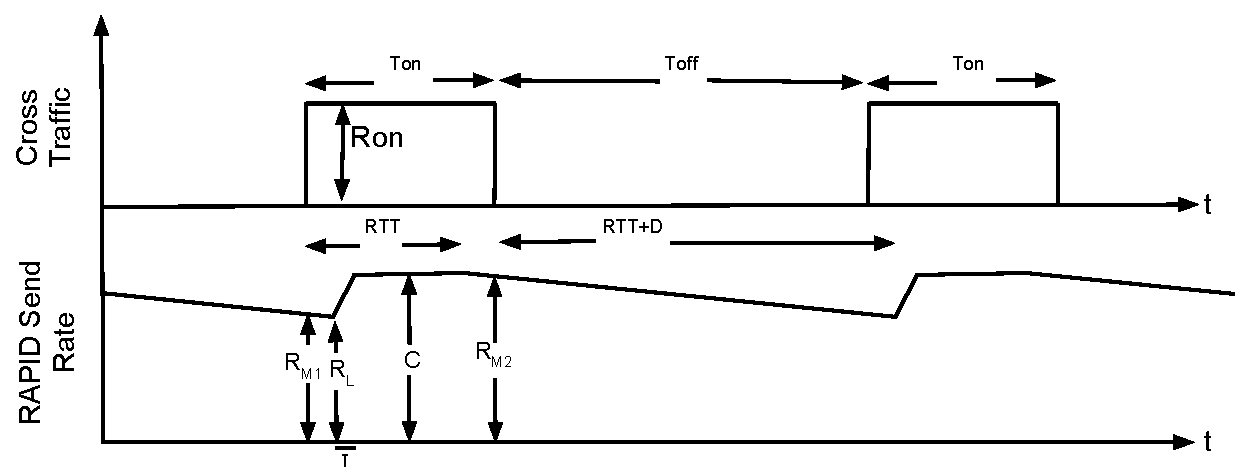
\includegraphics[width=0.9\textwidth]{img/small-burst1.pdf}
      \caption{Small-scale burst}
      \label{small1}
    \end{figure}

    The following set of inequalities also have to be true in order for the 
    particular case shown in Figure \ref{small1} to occur:
    \begin{IEEEeqnarray}{rCl}
      RTT & < & T_{on} \\
      RTT & \ge & T_{off} - D \\
      RTT & < & T_{on} + T_{off} - D - \tau
    \end{IEEEeqnarray}
    
    From Figure \ref{small1} we can derive expressions for $D$, $R_{M1}$, 
    $R_{M2}$, and $R_L$:
    \begin{IEEEeqnarray}{rCl}
      D & = & \frac{Q}{C} \nonumber \\
      D & = & \frac{(R_{M1} - 2C + R_L + 2R_{on})(RTT + D - T_{off})}{2C} 
        + \frac{(R_L - C + 2 R_{on}) \tau}{2C}  \nonumber \\
        && + \frac{R_{on} ( T_{off} - D - \tau)}{C}  + 
        \frac{(2 R_{on} + R_{M2} - C) (T_{on} - RTT)}{2C} \label{dsmall1} \\
      R_{M1} & = & C + \frac{R_{on} (RTT - T_{off} - T_{on})}{\eta} 
      \label{rm1small1} \\
      R_{M2} & = & C + \frac{R_{on} (RTT - T_{on})}{\eta} 
      \label{rm2small1}\\
      R_L & = & C - \frac{R_{on} ( T_{on} + D )}{\eta} \label{rlsmall1}
    \end{IEEEeqnarray}

    Using equations \eqref{rsmall1}, \eqref{dsmall1}, \eqref{rm1small1}, 
    \eqref{rm2small1}, and \eqref{rlsmall1} we can derive an expression for 
    the Rapid throughput $R$ as a function of $T_{on}$, $T_{off}$, $R_{on}$, 
    $C$, $\tau$, $\eta$, and $RTT$.

    \item When Rapid does not have enough time to increase its sending rate to 
    $C$ but has enough time to decrease its sending rate to $C - R_{on}$ the 
    following equations are true:
    \begin{IEEEeqnarray}{rCl}
      T_{off} - D < \tau \label{tau2} \\
      T_{on} + D \ge \eta \label{eta2}
    \end{IEEEeqnarray}

    Figure \ref{small2} shows plots of the Rapid send rate and the cross 
    traffic send rate when inequalities \eqref{tau2} and \eqref{eta2} are 
    true. In the figure, $D$ is the queueing delay, $R_H$ is the highest 
    sending rate, $R_{M1}$ is the instantaneous send rate of Rapid when the 
    cross traffic burst begins, and $R_{M2}$ is the instantaneous send rate of 
    Rapid when the cross traffic ends. For these cases, the Rapid throughput 
    can be expressed as
    \begin{IEEEeqnarray}{rCl}
      R & = & \left ( \frac{R_H + C - R_{on}}{2} \right ) \left ( \frac{T_{off} 
      - D + \eta}{T_{on} + T_{off}} \right ) \nonumber \\
      && + (C - R_{on}) \frac{T_{on} + D - \eta}{T_{on} + T_{off}}
      \label{rsmall2}
    \end{IEEEeqnarray}
    
    \begin{figure}[h]
      \centering
      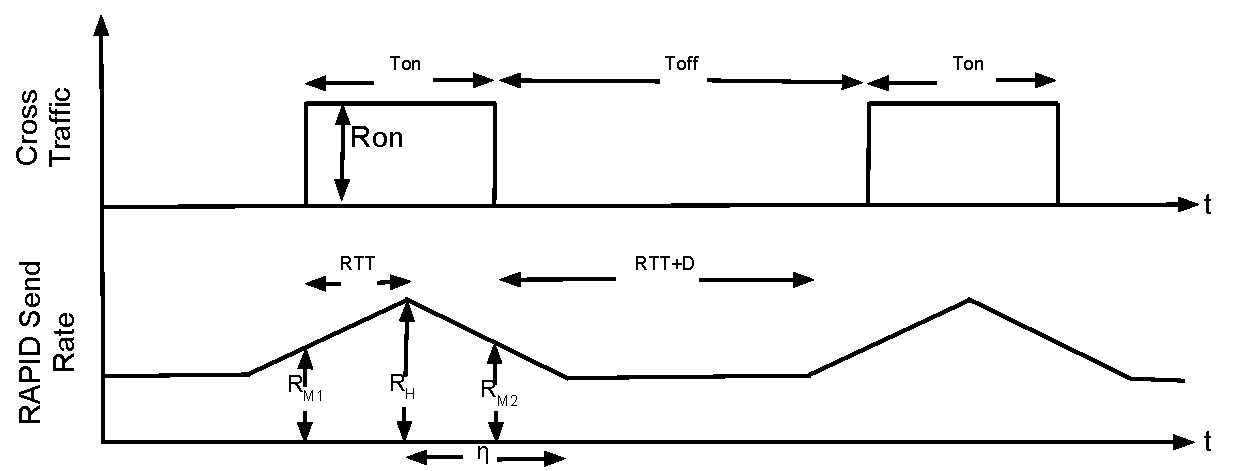
\includegraphics[width=0.9\textwidth]{img/small-burst2.pdf}
      \caption{Small-scale burst}
      \label{small2}
    \end{figure}

    The following set of inequalities also have to be true in order for the 
    particular case shown in Figure \ref{small2} to occur:
    \begin{IEEEeqnarray}{rCl}
      RTT & < & T_{on} \\
      RTT & \ge & T_{on} - \eta \\
      RTT & < & T_{on} + T_{off} - \eta \\
      RTT & < & T_{off} - D
    \end{IEEEeqnarray}

    From Figure \ref{small2} we can derive expressions for $D$, $R_{M1}$, 
    $R_{M2}$, and $R_H$:
    \begin{IEEEeqnarray}{rCl}
      D & = & \frac{Q}{C} \nonumber \\
      D & = & \frac{RTT (R_{M1} - 2 C + 2 R_{on} + R_H)}{2 C} \nonumber \\
      && + \frac{(T_{on} - RTT)(R_H - 2 C + 2 R_{on} + R_{M2})}{2 C} 
      \label{dsmall2} \\
      R_{M1} & = & C + \frac{R_{on} (T_{off} - \tau - D - RTT)}{\tau}
      \label{rm1small2} \\
      R_{M2} & = & R_H + \frac{RTT ( R_H + R_{on} - C ) + T_{on} ( C - R_H - 
      R_{on})}{\eta} 
      \label{rm2small2} \\
      R_H & = & C + \frac{R_{on} (T_{off} - \tau - D)}{\tau}
      \label{rhsmall2}
    \end{IEEEeqnarray}

    Using equations \eqref{rsmall2}, \eqref{dsmall2}, \eqref{rm1small2}, 
    \eqref{rm2small2}, and \eqref{rhsmall2} we can obtain an expression for 
    the Rapid throughput $R$ as a function of $T_{on}$, $T_{off}$, $R_{on}$, 
    $C$, $\tau$, $\eta$, and $RTT$.

    \item When Rapid does not have enough time to increase its sending rate to 
    $C$ and does not have enough time to decrease its sending rate to 
    $C - R_{on}$ the following equations are true:
    \begin{IEEEeqnarray}{rCl}
      T_{off} - D & < & \tau \label{tau3} \\
      T_{on} + D & < & \eta \label{eta3}
    \end{IEEEeqnarray}

    Figure \ref{small3} shows plots of the Rapid send rate and the cross 
    traffic send rate when inequalities \eqref{tau3} and \eqref{eta3} are 
    true. In figure, $D$ is the queueing delay, $R_L$ is the lowest sending 
    rate, $R_H$ is the highest sending rate, $R_{M1}$ is the instantaneous 
    send rate of Rapid when the cross traffic burst begins, and $R_{M2}$ is 
    the instantaneous send rate of Rapid when the cross traffic ends. For 
    these cases, the Rapid throughput can be expressed as
    \begin{equation}
      R = \frac{R_L + R_H}{2}
      \label{rsmall3}
    \end{equation}
    
    \begin{figure}[h]
      \centering
      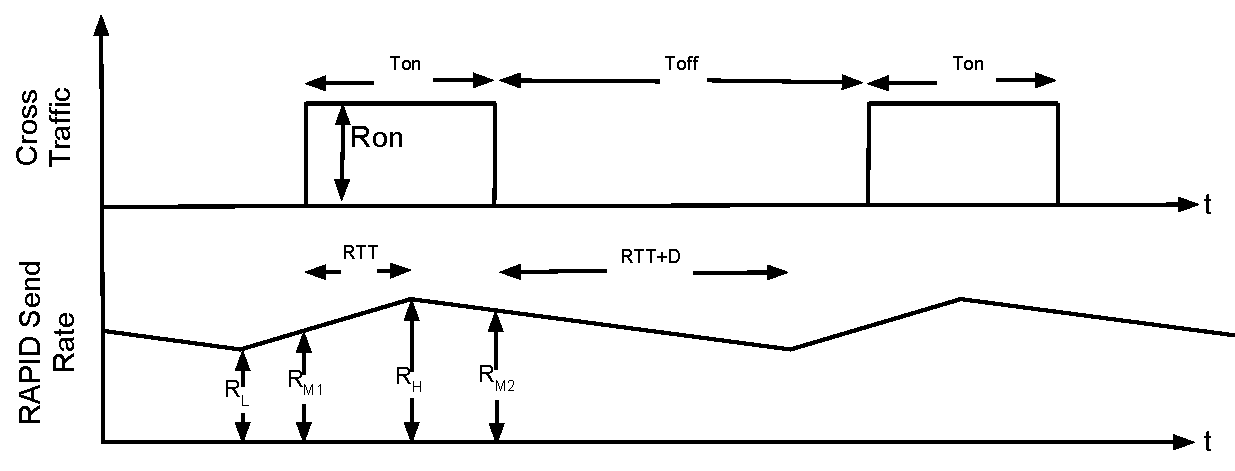
\includegraphics[width=0.9\textwidth]{img/small-burst3.pdf}
      \caption{Small-scale burst}
      \label{small3}
    \end{figure}

    The following set of inequalities also have to be true in order for the 
    particular case shown in Figure \ref{small3} to occur:
    \begin{IEEEeqnarray}{rCl}
      RTT & < & T_{on} \\
      RTT & < & T_{off} - D \\
    \end{IEEEeqnarray}

    From Figure \ref{small3} we can derive expressions for $D$, $R_{M1}$, 
    $R_{M2}$, $R_L$, and $R_H$:
    \begin{IEEEeqnarray}{rCl}
      D & = & \frac{Q}{C} \nonumber \\
      D & = & \frac{RTT(R_{M1} - 2 C + 2 R_{on} + R_H)}{2} \nonumber \\
      && + \frac{(T_{on} - RTT) (R_H - 2 C + 2 R_{on} + R_{M2})}{2} 
      \label{dsmall3} \\
      R_{M1} & = & R_L + \frac{R_L (D + RTT - T_{off}) + C(T_{off} - RTT - D)}
      {\tau} 
      \label{rm1small3} \\
      R_{M2} & = & R_H + \frac{RTT(R_H + R_{on} - C) + T_{on} (C - R_H - 
      R_{on})}{\eta} 
      \label{rm2small3} \\
      R_L & = & R_H - (R_H - (C - R_{on})) \left(\frac{T_{on} + D}{\eta} 
      \right ) 
      \label{rlsmall3} \\
      R_h & = & R_L + (C - R_L) \left (\frac{T_{off} - D}{\tau} \right )
      \label{rhsmall3}
    \end{IEEEeqnarray}

    Using equations \eqref{rsmall3}, \eqref{dsmall3}, \eqref{rm1small3}, 
    \eqref{rm2small3}, \eqref{rlsmall3}, and \eqref{rhsmall3} we can derive 
    an expression for the Rapid throughput $R$ as a function of $T_{on}$, 
    $T_{off}$, $R_{on}$, $C$, $\tau$, $\eta$, and $RTT$.

  \end{enumerate}
